\section{Data Model}
\label{sec:data-model}

The codetopo database schema consists of six principal tables and three FTS
virtual tables. This section describes each table, the relationships between
them, and the FTS indexing strategy~\cite{hipp2014fts5}.

\begin{figure}[htbp]
\centering
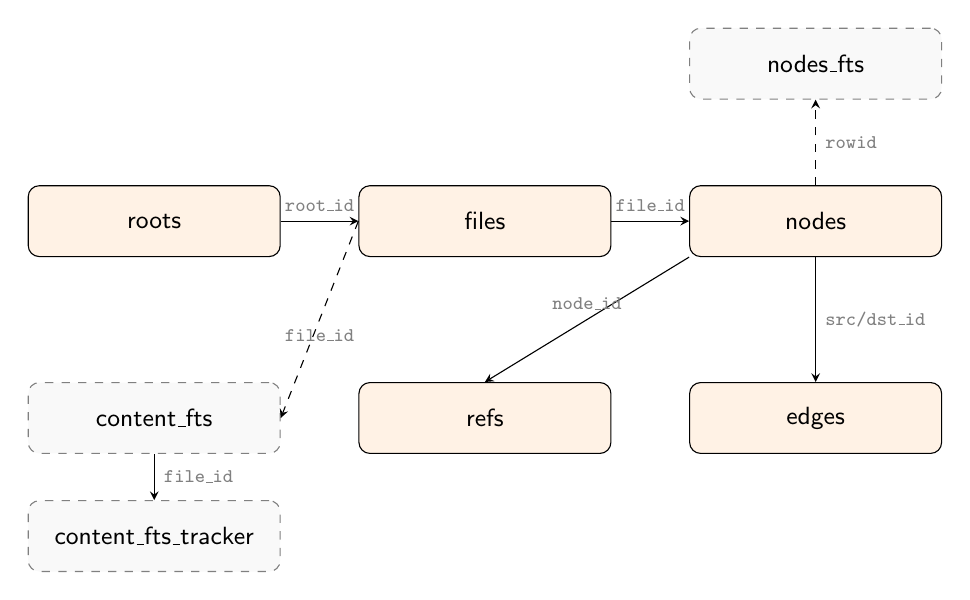
\begin{tikzpicture}[
  entity/.style={draw, fill=orange!10, rounded corners,
                 minimum width=3.2cm, minimum height=0.9cm,
                 text centered, font=\small\sffamily},
  fts/.style={draw=gray, dashed, fill=gray!5, rounded corners,
              minimum width=3.2cm, minimum height=0.9cm,
              text centered, font=\small\sffamily},
  attr/.style={font=\scriptsize\ttfamily, text=gray},
  >=stealth
]
\node[entity] (roots)   at (-4.2, 0)   {roots};
\node[entity] (files)   at ( 0,   0)   {files};
\node[entity] (nodes)   at ( 4.2, 0)   {nodes};
\node[entity] (edges)   at ( 4.2,-2.5) {edges};
\node[entity] (refs)    at ( 0,  -2.5) {refs};
\node[fts]    (nfts)    at ( 4.2, 2.0) {nodes\_fts};
\node[fts]    (cfts)    at (-4.2,-2.5) {content\_fts};
\node[fts]    (ctrk)    at (-4.2,-4.0) {content\_fts\_tracker};

\draw[->] (roots)  -- node[attr,above]{\scriptsize root\_id} (files);
\draw[->] (files)  -- node[attr,above]{\scriptsize file\_id} (nodes);
\draw[->] (nodes.south) -- node[attr,right]{\scriptsize src/dst\_id} (edges.north);
\draw[->] (nodes.south west) -- node[attr,above]{\scriptsize node\_id} (refs.north);
\draw[->, dashed] (nodes.north) -- node[attr,right]{\scriptsize rowid} (nfts.south);
\draw[->, dashed] (files.west)  -- node[attr,below]{\scriptsize file\_id} (cfts.east);
\draw[->] (cfts.south) -- node[attr,right]{\scriptsize file\_id} (ctrk.north);
\end{tikzpicture}
\caption{Entity-relationship overview of the codetopo schema. Dashed arrows
         indicate FTS virtual-table relationships.}
\label{fig:schema}
\end{figure}

\subsection{roots}

\begin{lstlisting}[language=sql]
CREATE TABLE roots (
  id       INTEGER PRIMARY KEY,
  path     TEXT    NOT NULL UNIQUE,  -- absolute, canonical path
  added_at INTEGER NOT NULL          -- Unix timestamp
);
\end{lstlisting}

Each row represents a workspace root. The \texttt{id} is used as the root
offset in the ID allocation scheme described in \S\ref{sec:workspace}.

In addition to the relational tables, the schema keeps build and repository
metadata in a small \texttt{kv} store accessed through
\texttt{set\_kv()}/\texttt{get\_kv()}; Figure~\ref{fig:schema-kv} sketches
representative entries.

\begin{figure}[htbp]
  \centering
  \tritonnext{width=0.82\textwidth}
\begin{triton}
hashmap
  title schema kv
  buckets 5
  bucket 0: schema_version->8
  bucket 1: indexer_version->2026.06, last_index_time->2026-06-28T12:48
  bucket 2: repo_root->workspace, language_coverage->13langs
  bucket 3: git_head->abc1234, git_branch->main
\end{triton}
  \caption{Representative \texttt{kv} metadata entries stored alongside the
           structural tables.}
  \label{fig:schema-kv}
\end{figure}

\subsection{files}

\begin{lstlisting}[language=sql]
CREATE TABLE files (
  id        INTEGER PRIMARY KEY,
  path      TEXT    NOT NULL,        -- path relative to root
  language  TEXT,
  root_id   INTEGER NOT NULL REFERENCES roots(id)
);
\end{lstlisting}

\subsection{nodes}

The \texttt{nodes} table stores both file-level nodes (\texttt{node\_type =
'file'}) and symbol-level nodes (\texttt{node\_type = 'symbol'}):

\begin{lstlisting}[language=sql]
CREATE TABLE nodes (
  id            INTEGER PRIMARY KEY,
  file_id       INTEGER NOT NULL REFERENCES files(id),
  node_type     TEXT    NOT NULL,   -- 'file' | 'symbol'
  kind          TEXT,               -- function|class|method|...
  name          TEXT,
  qualname      TEXT,               -- fully-qualified name
  signature     TEXT,
  span          TEXT,               -- "start_line:start_col-end_line:end_col"
  is_definition INTEGER DEFAULT 1,
  visibility    TEXT,               -- public|private|protected|...
  doc           TEXT,               -- leading docstring
  stable_key    TEXT                -- language-specific stable identifier
);
\end{lstlisting}

\subsubsection{Symbol kinds}

The \texttt{kind} field takes one of: \texttt{function}, \texttt{method},
\texttt{class}, \texttt{struct}, \texttt{enum}, \texttt{enum\_variant},
\texttt{type\_alias}, \texttt{interface}, \texttt{trait}, \texttt{variable},
\texttt{constant}, \texttt{module}, \texttt{namespace}, \texttt{macro}.

\subsection{edges}

\begin{lstlisting}[language=sql]
CREATE TABLE edges (
  id         INTEGER PRIMARY KEY,
  src_id     INTEGER REFERENCES nodes(id),
  dst_id     INTEGER REFERENCES nodes(id),
  dst_name   TEXT,     -- unresolved callee name (approx edges)
  kind       TEXT NOT NULL,
  file_id    INTEGER REFERENCES files(id),
  confidence REAL DEFAULT 1.0
);
\end{lstlisting}

Edges with \texttt{confidence} below 0.3 are discarded at extraction time.

\subsubsection{Edge kinds}

\begin{description}
  \item[\texttt{calls}] A function or method call from \texttt{src} to \texttt{dst}.
  \item[\texttt{includes}] A module import or \texttt{\#include}.
  \item[\texttt{inherits}] A class or struct extending or implementing another.
  \item[\texttt{references}] A general reference that does not fit a more
        specific kind.
  \item[\texttt{contains}] A structural containment edge (e.g., method
        contained in a class).
\end{description}

\subsection{refs}

The \texttt{refs} table records finer-grained reference sites than edges:

\begin{lstlisting}[language=sql]
CREATE TABLE refs (
  id      INTEGER PRIMARY KEY,
  node_id INTEGER REFERENCES nodes(id),
  kind    TEXT NOT NULL,
  file_id INTEGER REFERENCES files(id),
  span    TEXT
);
\end{lstlisting}

Reference kinds: \texttt{call}, \texttt{type\_ref}, \texttt{include},
\texttt{inherit}, \texttt{field\_access}, \texttt{other}.

\subsection{FTS indexes}

Three FTS-related tables are maintained~\cite{hipp2014fts5}:

\paragraph{nodes\_fts.}  A standard FTS5 content-shadow table over the
\texttt{nodes} table:

\begin{lstlisting}[language=sql]
CREATE VIRTUAL TABLE nodes_fts USING fts5(
  name, qualname, signature, doc,
  content='nodes', content_rowid='id'
);
\end{lstlisting}

This is used by \texttt{symbol\_search} for BM25-ranked prefix queries over
symbol names, qualified names, signatures, and docstrings.

\paragraph{content\_fts.}  A \emph{contentless}\footnote{A \texttt{content=}
FTS5 table mirrors the original rows in its shadow tables, enabling
snippet generation from stored data, but it doubles storage --- every indexed
string is kept both in the shadow table and on disk. The contentless variant
(\texttt{content=''}) stores only the inverted index, halving storage at the
cost of requiring the source file to be re-read for result display. This
trade-off is acceptable because source files are always present locally.}
FTS5 table with the trigram
tokenizer, indexed per source line:

\begin{lstlisting}[language=sql]
CREATE VIRTUAL TABLE content_fts USING fts5(
  line_text,
  file_id UNINDEXED,
  line_no  UNINDEXED,
  content='',
  tokenize='trigram'
);
\end{lstlisting}

Because this table is contentless (it does not store the original text),
it cannot be scanned for its row contents. Results are retrieved by matching
on \texttt{line\_text} and then reading the actual source from disk.

\paragraph{content\_fts\_tracker.}  A plain table that tracks which files
have been indexed into \texttt{content\_fts}, since the FTS table itself
cannot be queried for its file coverage:

\begin{lstlisting}[language=sql]
CREATE TABLE content_fts_tracker (
  file_id INTEGER PRIMARY KEY REFERENCES files(id)
);
\end{lstlisting}

\subsection{Multi-root ID scheme}

All nodes across all workspace roots share a single \texttt{nodes} table. To
keep IDs globally unique, codetopo uses a multiplicative offset\footnote{The
factor $10^9$ was chosen for readability in debug output: root 1's IDs begin
at \texttt{1\,000\,000\,001}. SQLite's 64-bit signed rowid ceiling
($2^{63}-1 \approx 9.2 \times 10^{18}$) accommodates up to $\sim$9.2 billion
root slots at this scale, far beyond any practical need.}:
\[
  \text{global\_id} = \text{root\_id} \times 10^9 + \text{local\_id}
\]
where \texttt{local\_id} is the SQLite autoincrement rowid within the root's
ID space ($1$ through $10^9 - 1$). This scheme supports up to $10^9 - 1$
symbols per root. The full scheme is described in \S\ref{sec:workspace}.
